% !TeX TXS-program:compile = txs:///pdflatex/[--shell-escape]

\documentclass[a4paper]{article}

\usepackage[utf8]{inputenc}
\usepackage[italian]{babel}

\usepackage{subfiles}
\usepackage{alertmessage}
\usepackage{svg}
\usepackage{graphicx}
\usepackage{subfig}
\usepackage{float}

\title{IR Extender}

\include{authors.tex}

\date{
    Aprile 2022 \endgraf\bigskip
    \bigskip\bigskip\bigskip\bigskip\bigskip
    Relazione in corso di scrittura
}

\begin{document}

\begin{titlepage}
\maketitle    
\end{titlepage}

\tableofcontents
\clearpage

\section{Introduzione}

Il seguente documento descrive come realizzare un IR Extender.

Il sistema e' formato da 3 componenti principali:

\includesvg[width=4in]{assets/ir_extender}

\begin{itemize}
    \item Ricevitore e Publisher MQTT: un NodeMCU e' collegato ad un ricevitore infrarossi e alla rete Wi-Fi.

        Il compito di questo dispositivo e' di:
        \begin{enumerate}
            \item Ricevere un segnale infrarossi da un telecomando.
            \item Inviare l'informazione del segnale infrarossi, utilizzando la rete Wi-Fi, con il protocollo MQTT al Broker MQTT.
        \end{enumerate}

        Nel contesto del sistema e' il ricevitore.
    
    \item Broker MQTT: un servizio in cloud gestito da HiveMQ.
    
        Il suo compito e':
        \begin{enumerate}
            \item Ricevere l'informazione proveniente dal Publisher MQTT.
            \item Inviare l'informazione MQTT al Subscriber MQTT.
        \end{enumerate}

        Nel sistema il suo ruolo e' da tramite tra il ricevitore e il trasmettitore.
    
    \item Trasmettitore e Subscriber MQTT: un altro NodeMCU e' collegato ad un trasmettitore infrarossi e alla rete Wi-Fi.
    
        Il compito di questo dispositivo e' di:
        \begin{enumerate}
            \item Ricevere l'informazione dal Broker MQTT
            \item Inviare un segnale infrarossi con l'informazione del Broker MQTT con il trasmettitore infrarossi
        \end{enumerate}

        Nel contesto del sistema e' il trasmettitore.

\end{itemize}

\alertinfo{Le reti Wi-Fi del ricevitore e del trasmettitore possono essere due reti differenti o la stessa rete.}
\alertinfo{Le 3 componenti comunicano mediante il protocollo MQTT.}

\section{Ricevitore}

Il dispositivo ricevitore si occupa di:
\begin{enumerate}
    \item Ricevere un segnale infrarossi da un telecomando.
    \item Inviare l'informazione del segnale infrarossi, utilizzando la rete Wi-Fi, con il protocollo MQTT al Broker MQTT.
\end{enumerate}

\begin{figure}[H]
    \centering
    \subfloat{{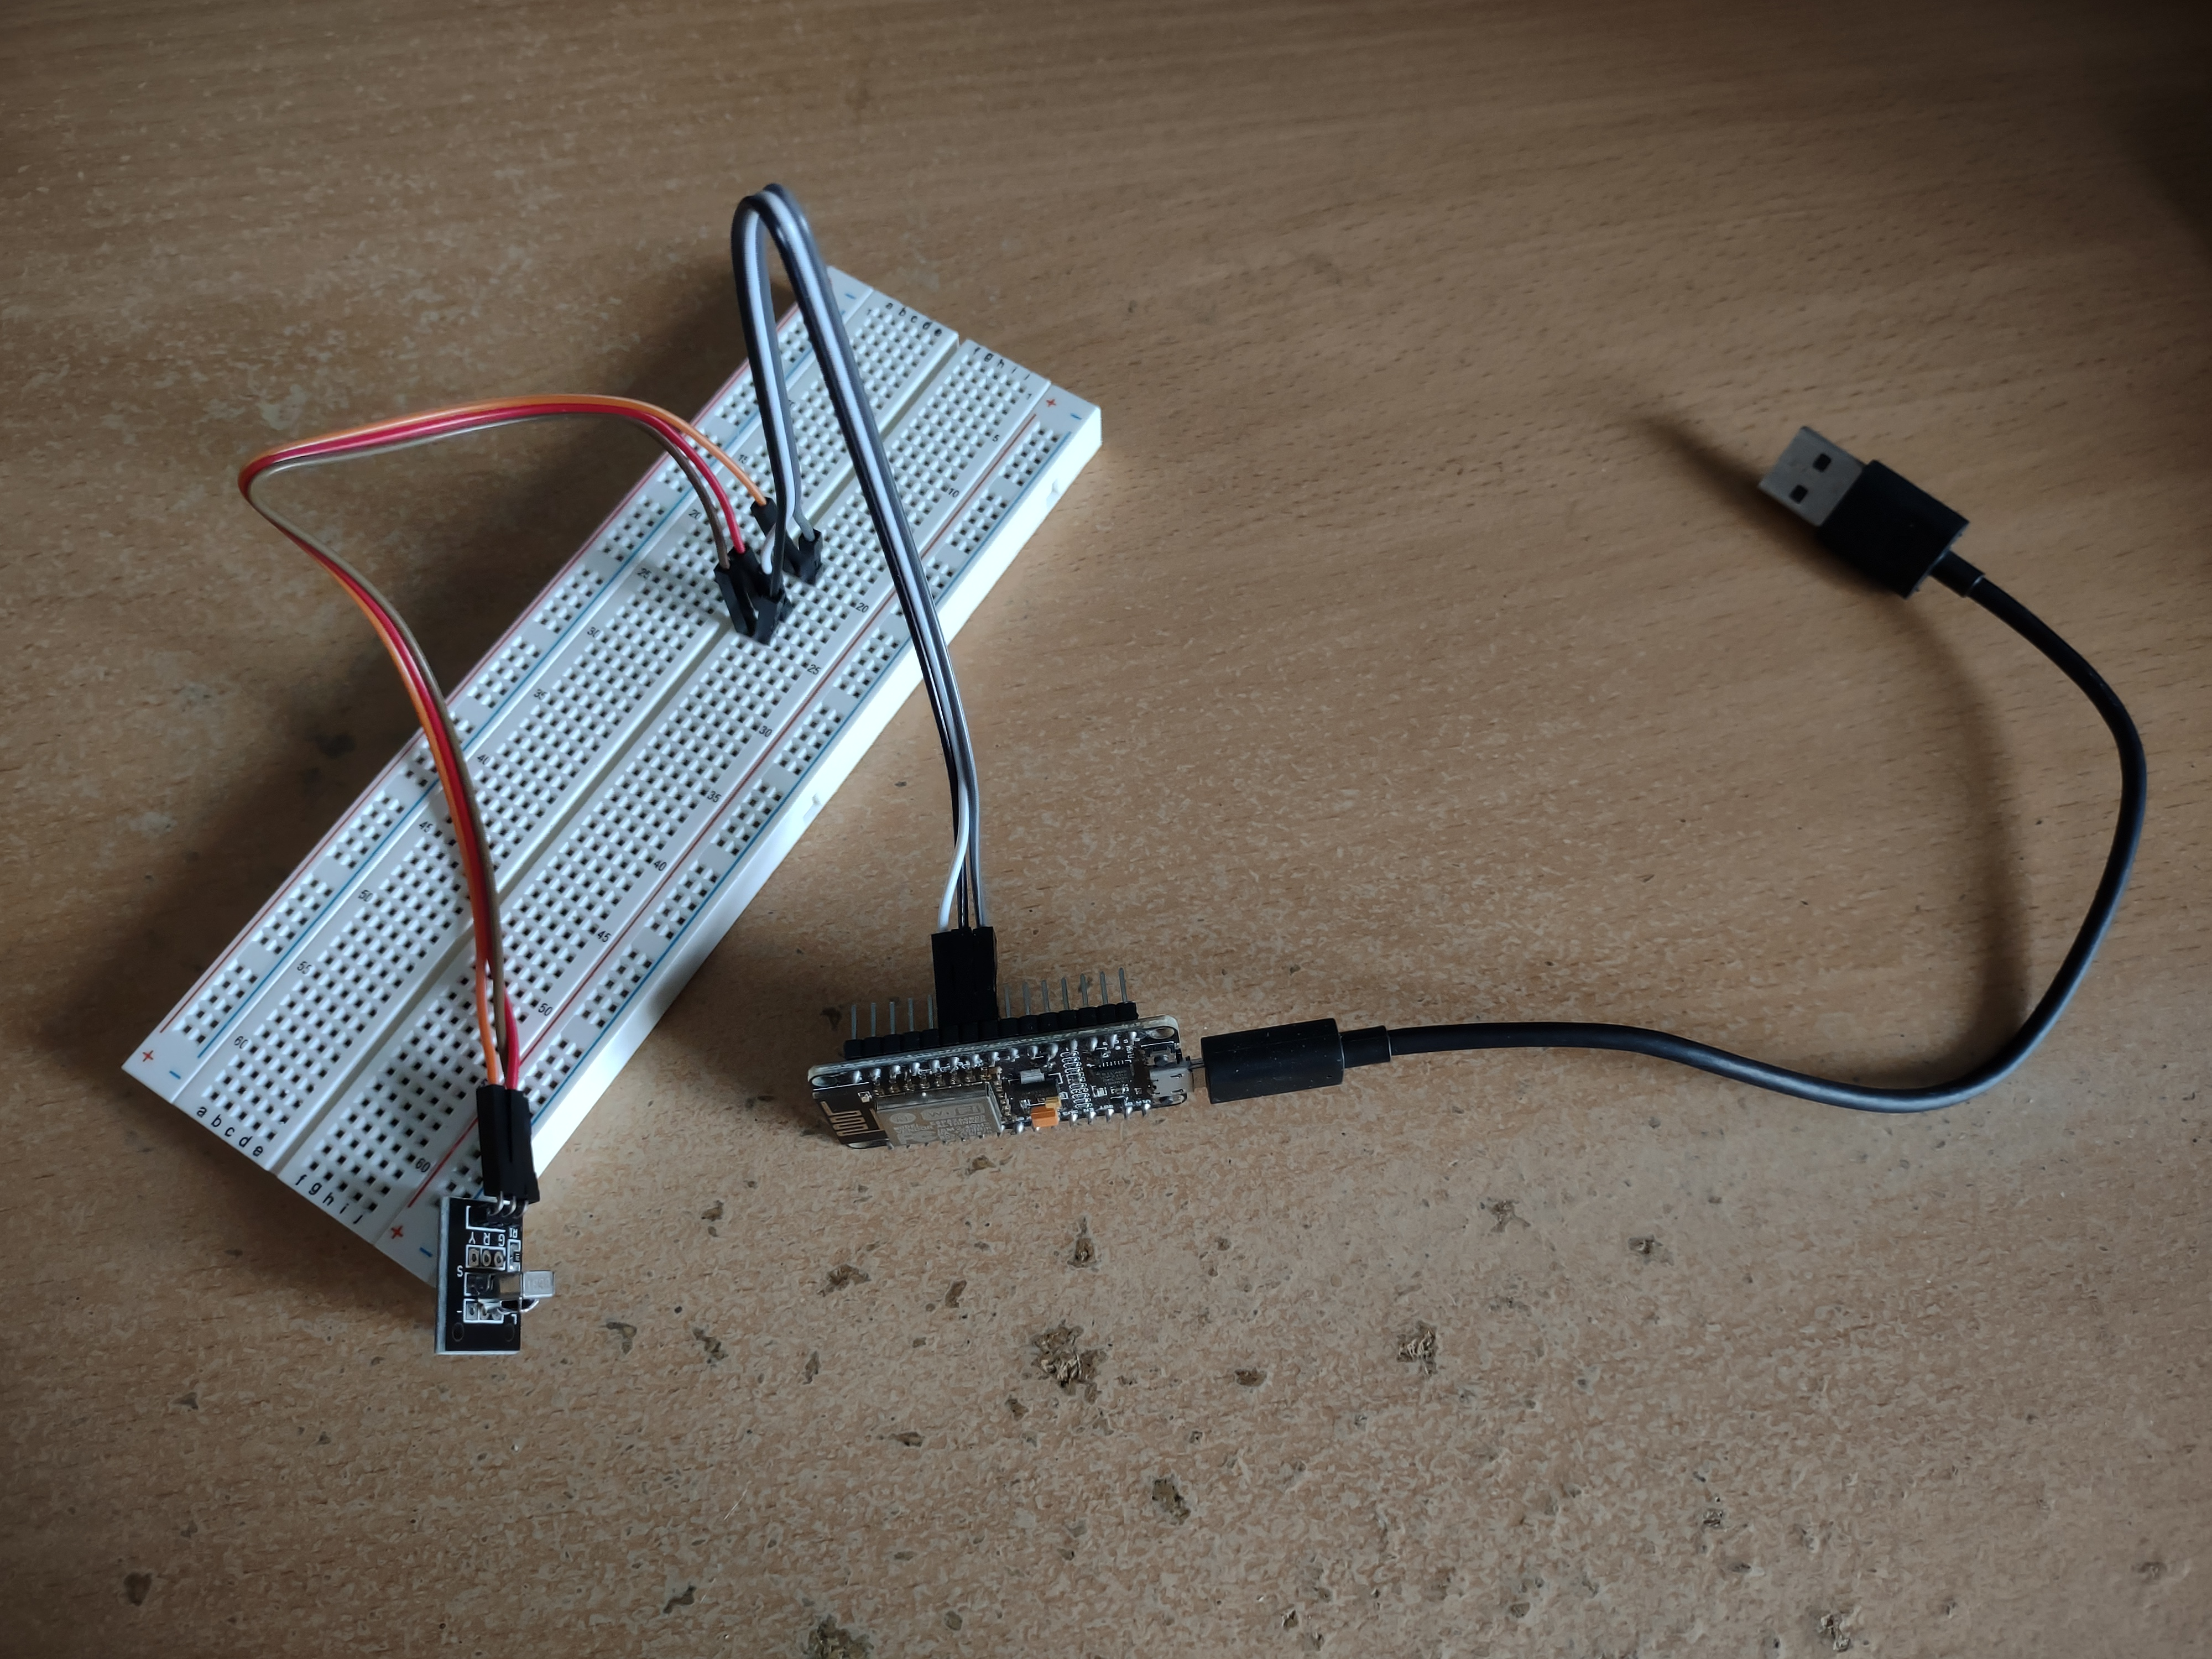
\includegraphics[width=5cm]{assets/receiver1} }}%
    \qquad
    \subfloat{{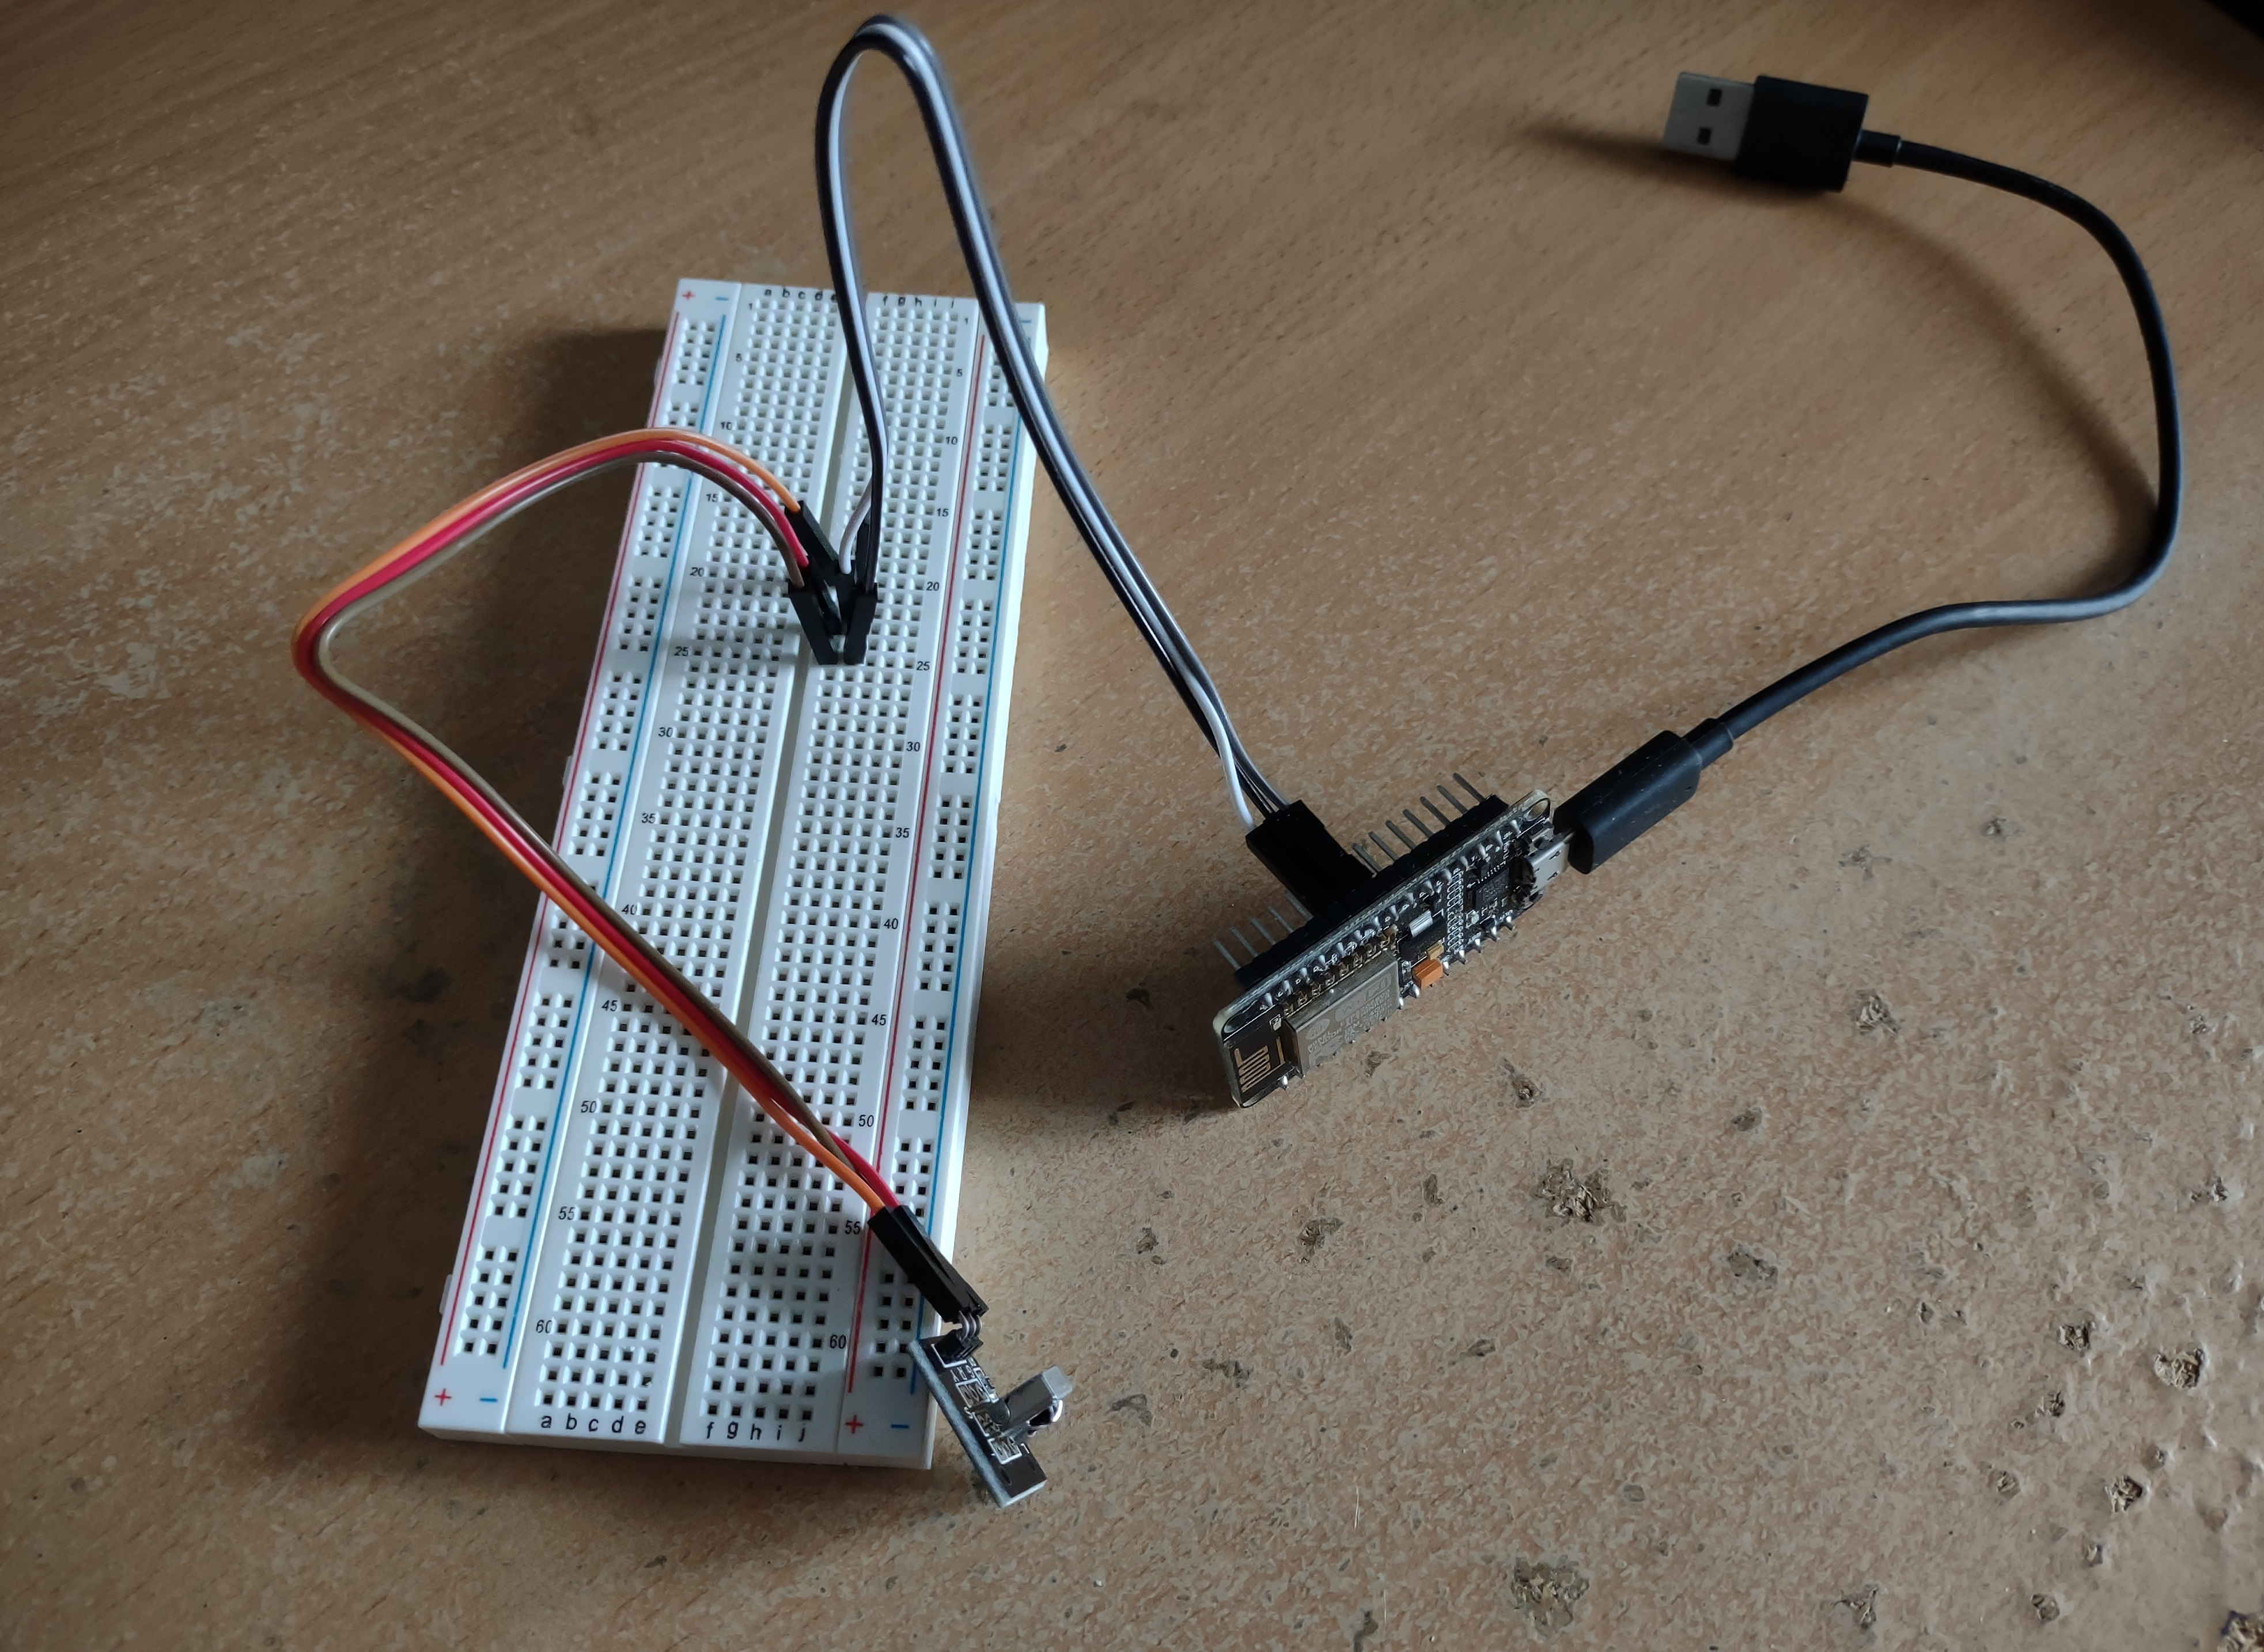
\includegraphics[width=5cm]{assets/receiver2} }}%
    \qquad
    \subfloat{{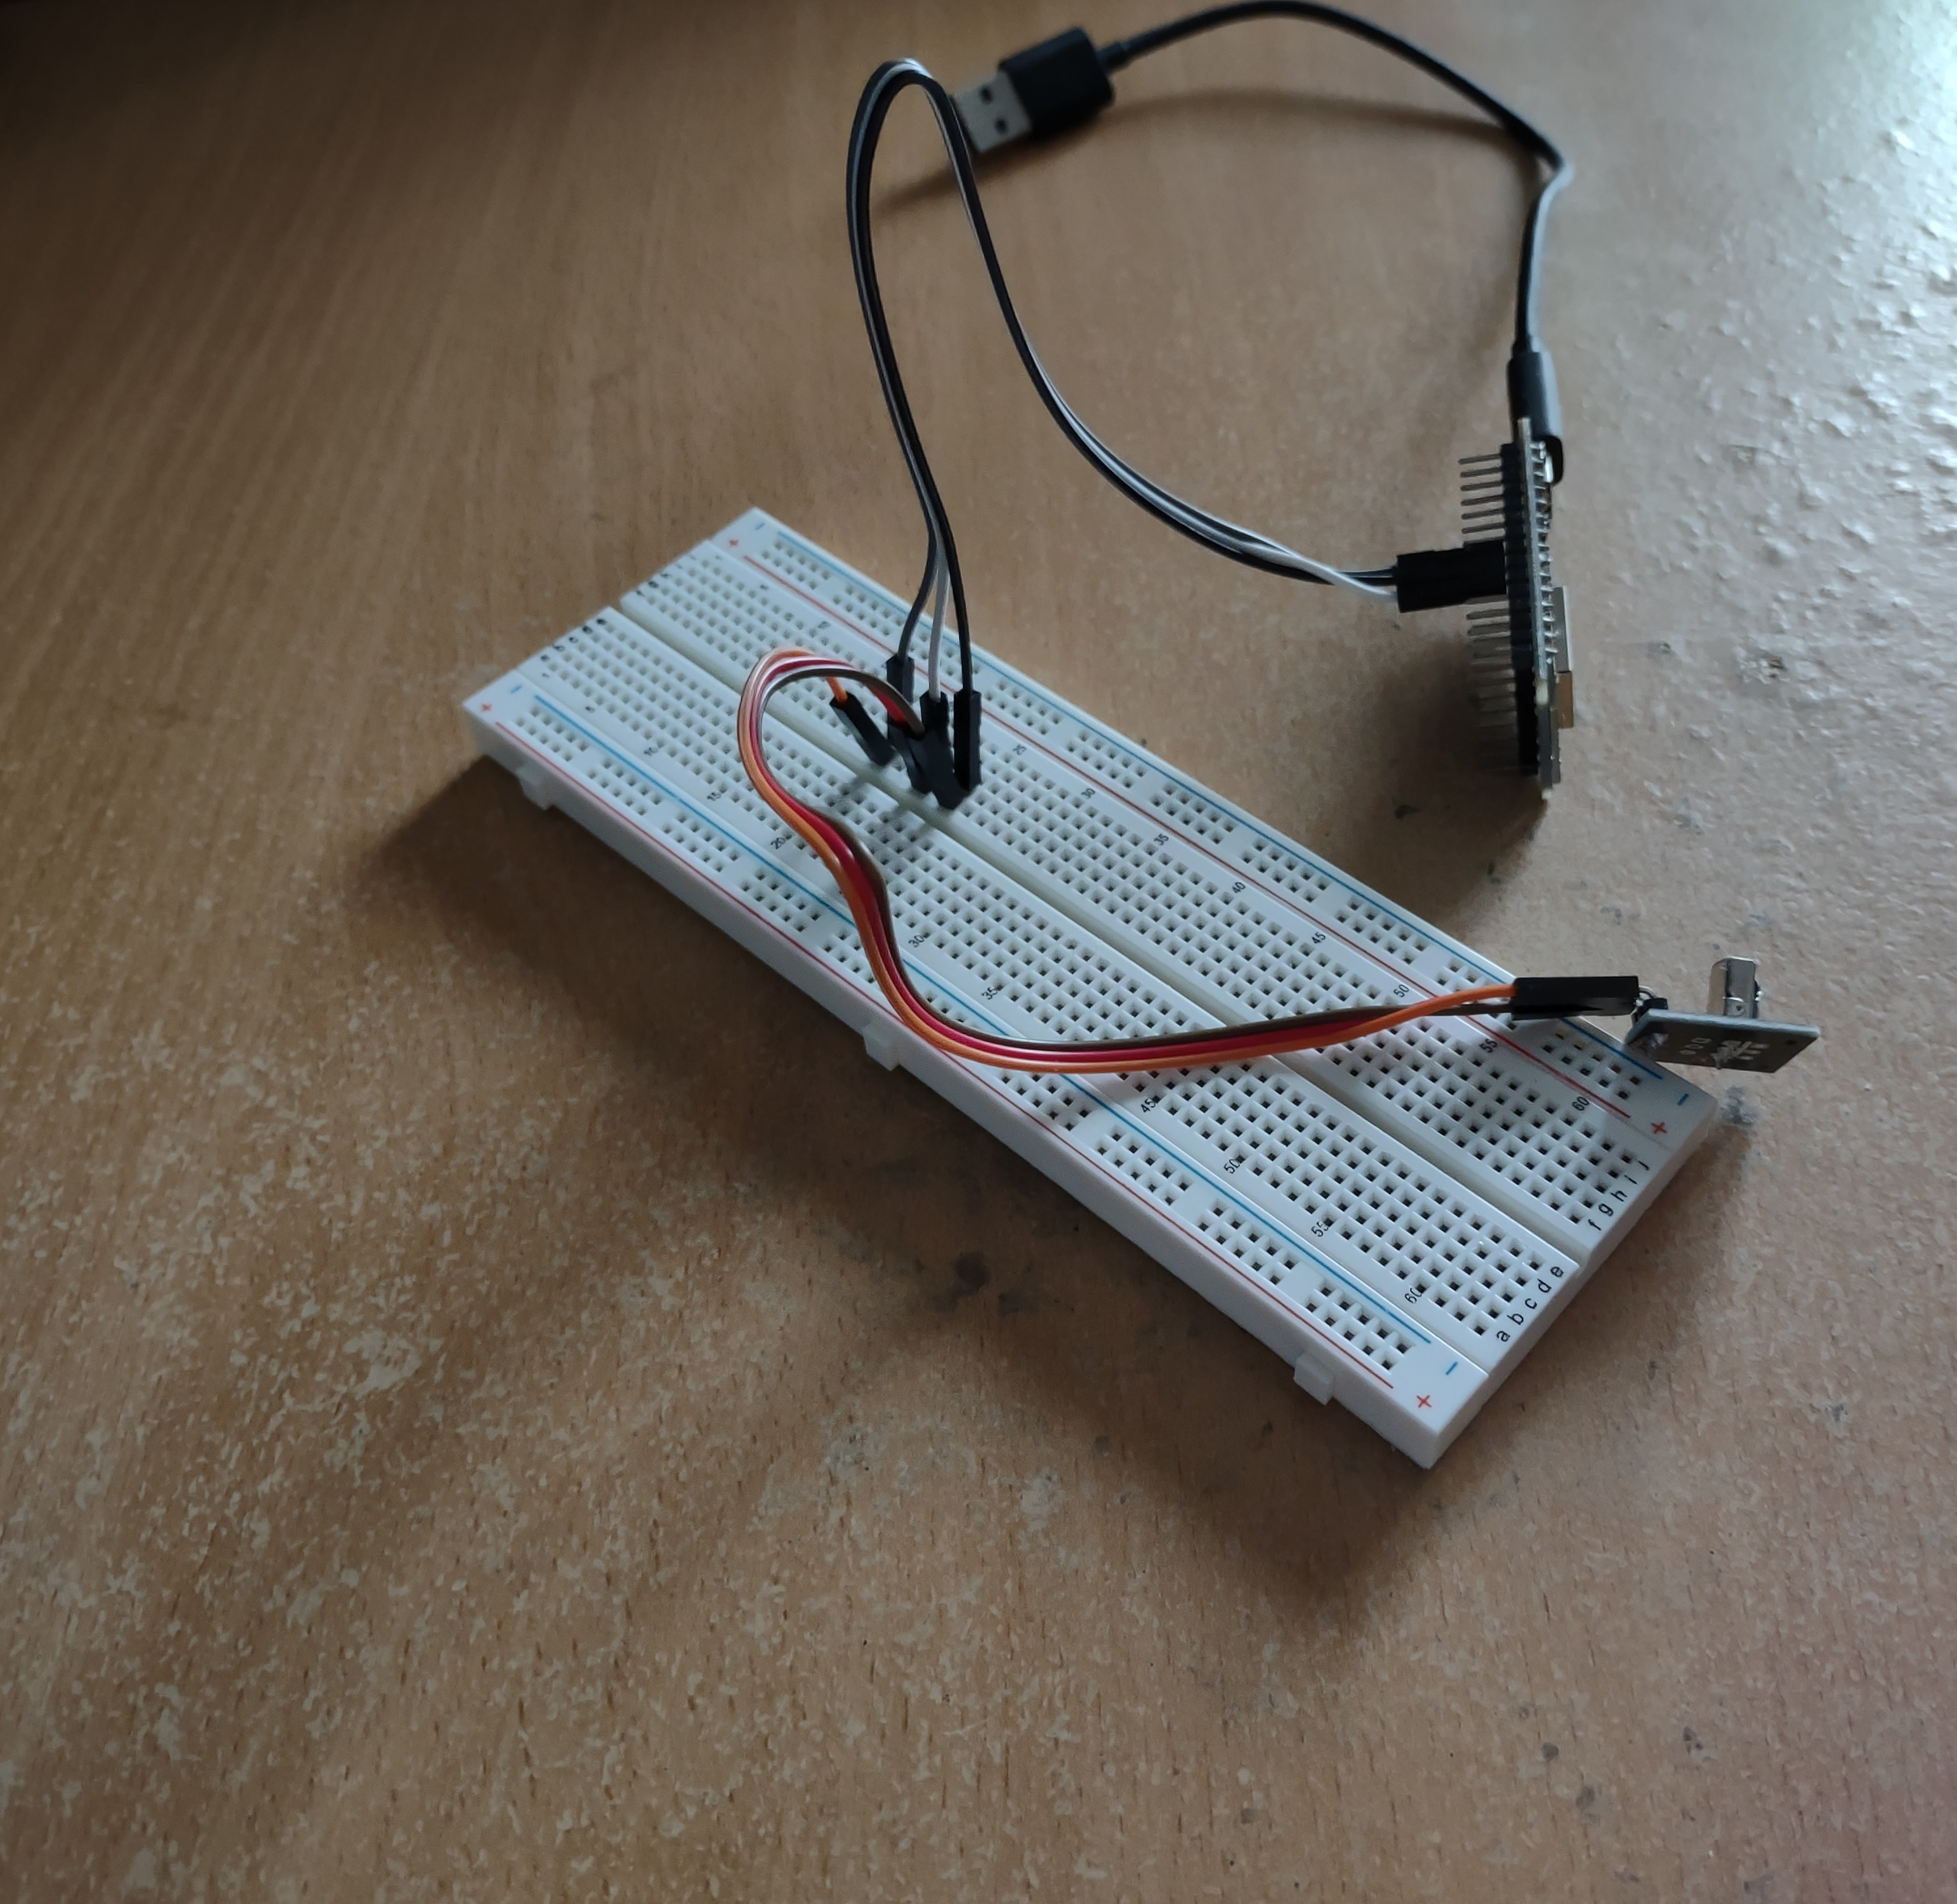
\includegraphics[width=5cm]{assets/receiver3} }}%
    \caption{Foto Ricevitore}%
    \label{fig:example}%
\end{figure}

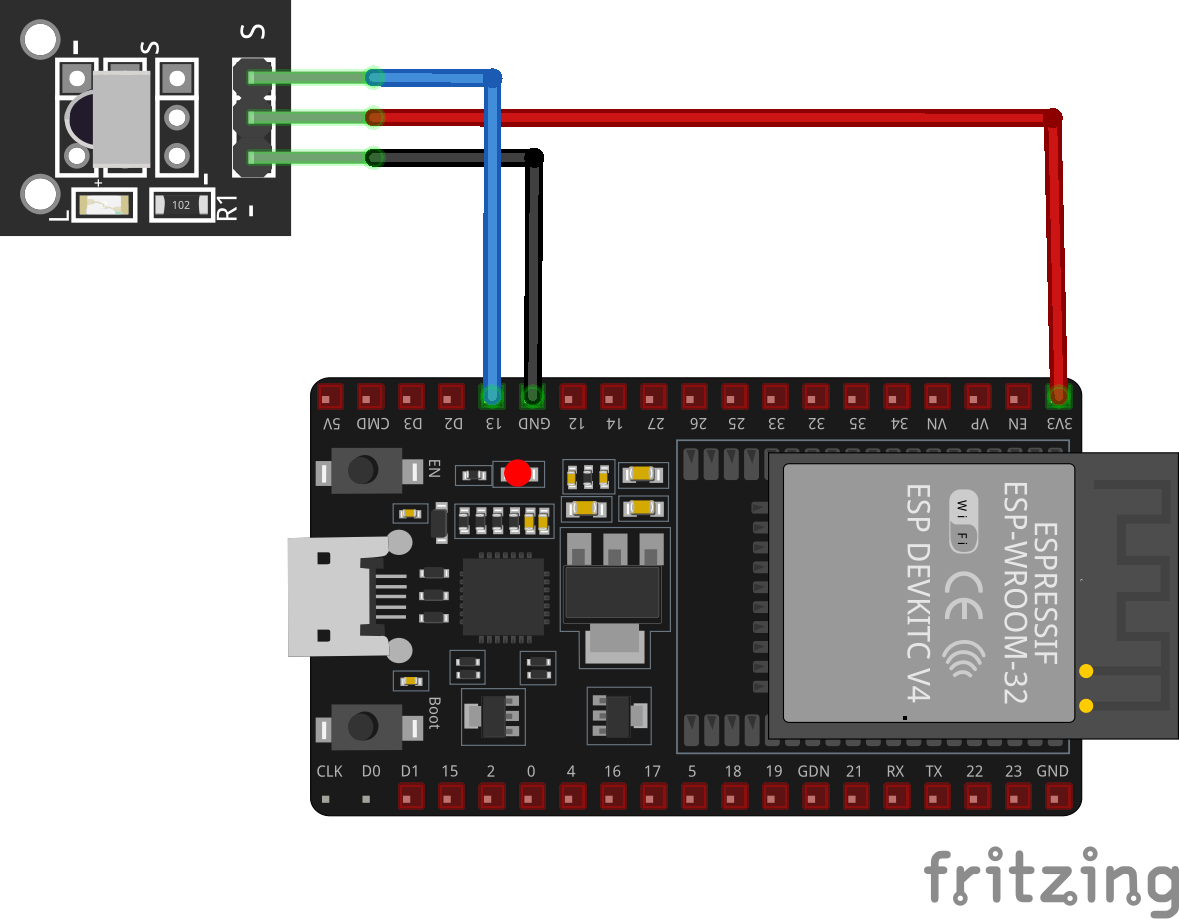
\includegraphics[width=\textwidth,height=\textheight,keepaspectratio]{assets/receiver_fritzing}

\section{Trasmettitore}
Il dispositivo trasmettitore si occupa di:

\begin{enumerate}
    \item Ricevere l'informazione dal Broker MQTT
    \item Inviare un segnale infrarossi con l'informazione del Broker MQTT con il trasmettitore infrarossi
\end{enumerate}

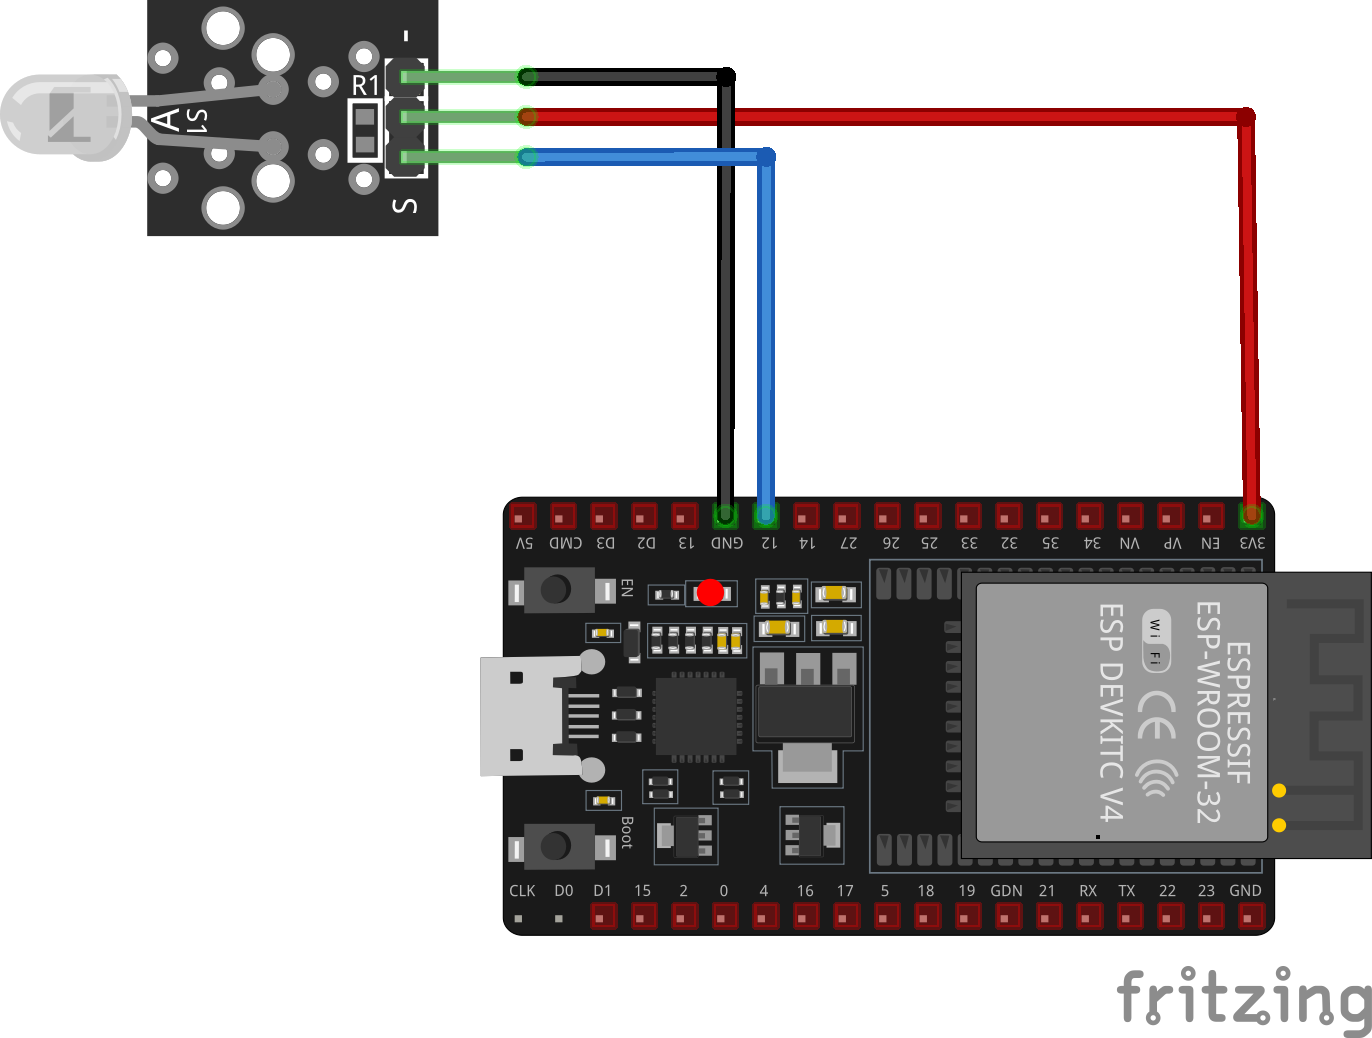
\includegraphics[width=\textwidth,height=\textheight,keepaspectratio]{assets/transmitter_fritzing}

\section{Broker MQTT}

Il compito del Broker MQTT e' di:
\begin{enumerate}
    \item Ricevere l'informazione proveniente dal Publisher MQTT.
    \item Inviare l'informazione MQTT ai Subscriber MQTT.
\end{enumerate}

Per creare un Broker MQTT e' necessario registrarsi, effettuare l'accesso e poi creare un nuovo cluster:

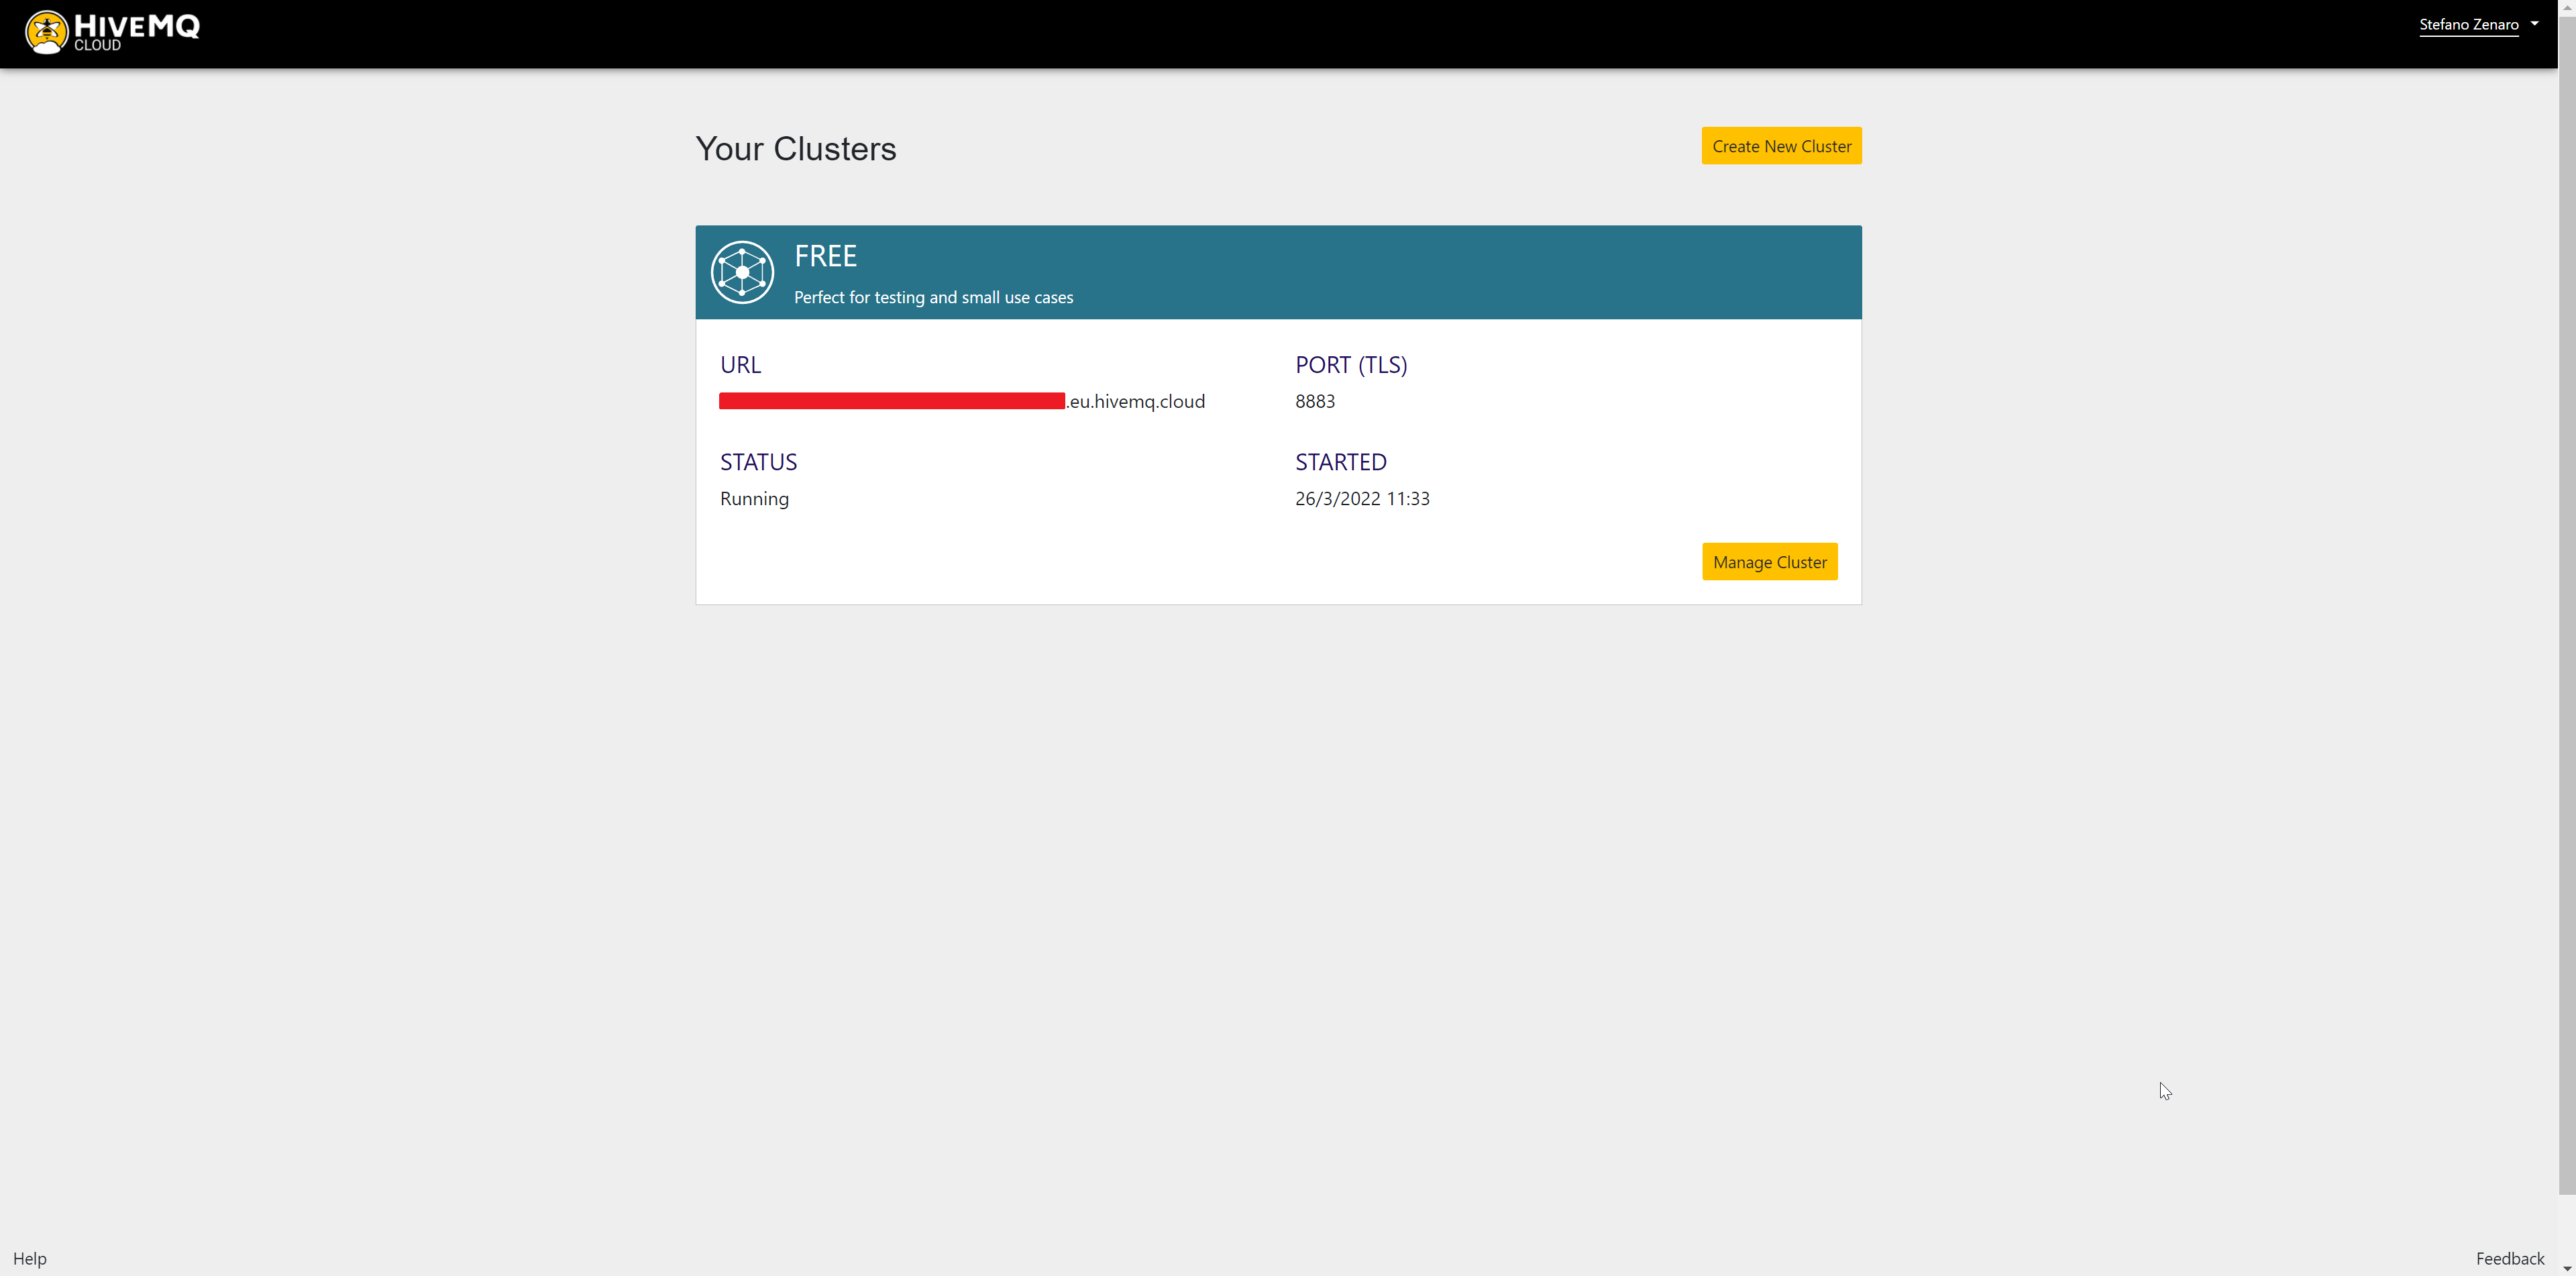
\includegraphics[width=\textwidth,height=\textheight,keepaspectratio]{assets/hivemq_clusters}

\alertinfo{Dalla schermata principale e' possibile creare nuovi cluster e visualizzare informazioni di stato tra cui l'URL e la porta del Broker MQTT.}

Cliccando su "manage cluster" e' possibile vedere le informazioni di stato precedenti piu' altre informazioni relative all'uso del cluster:

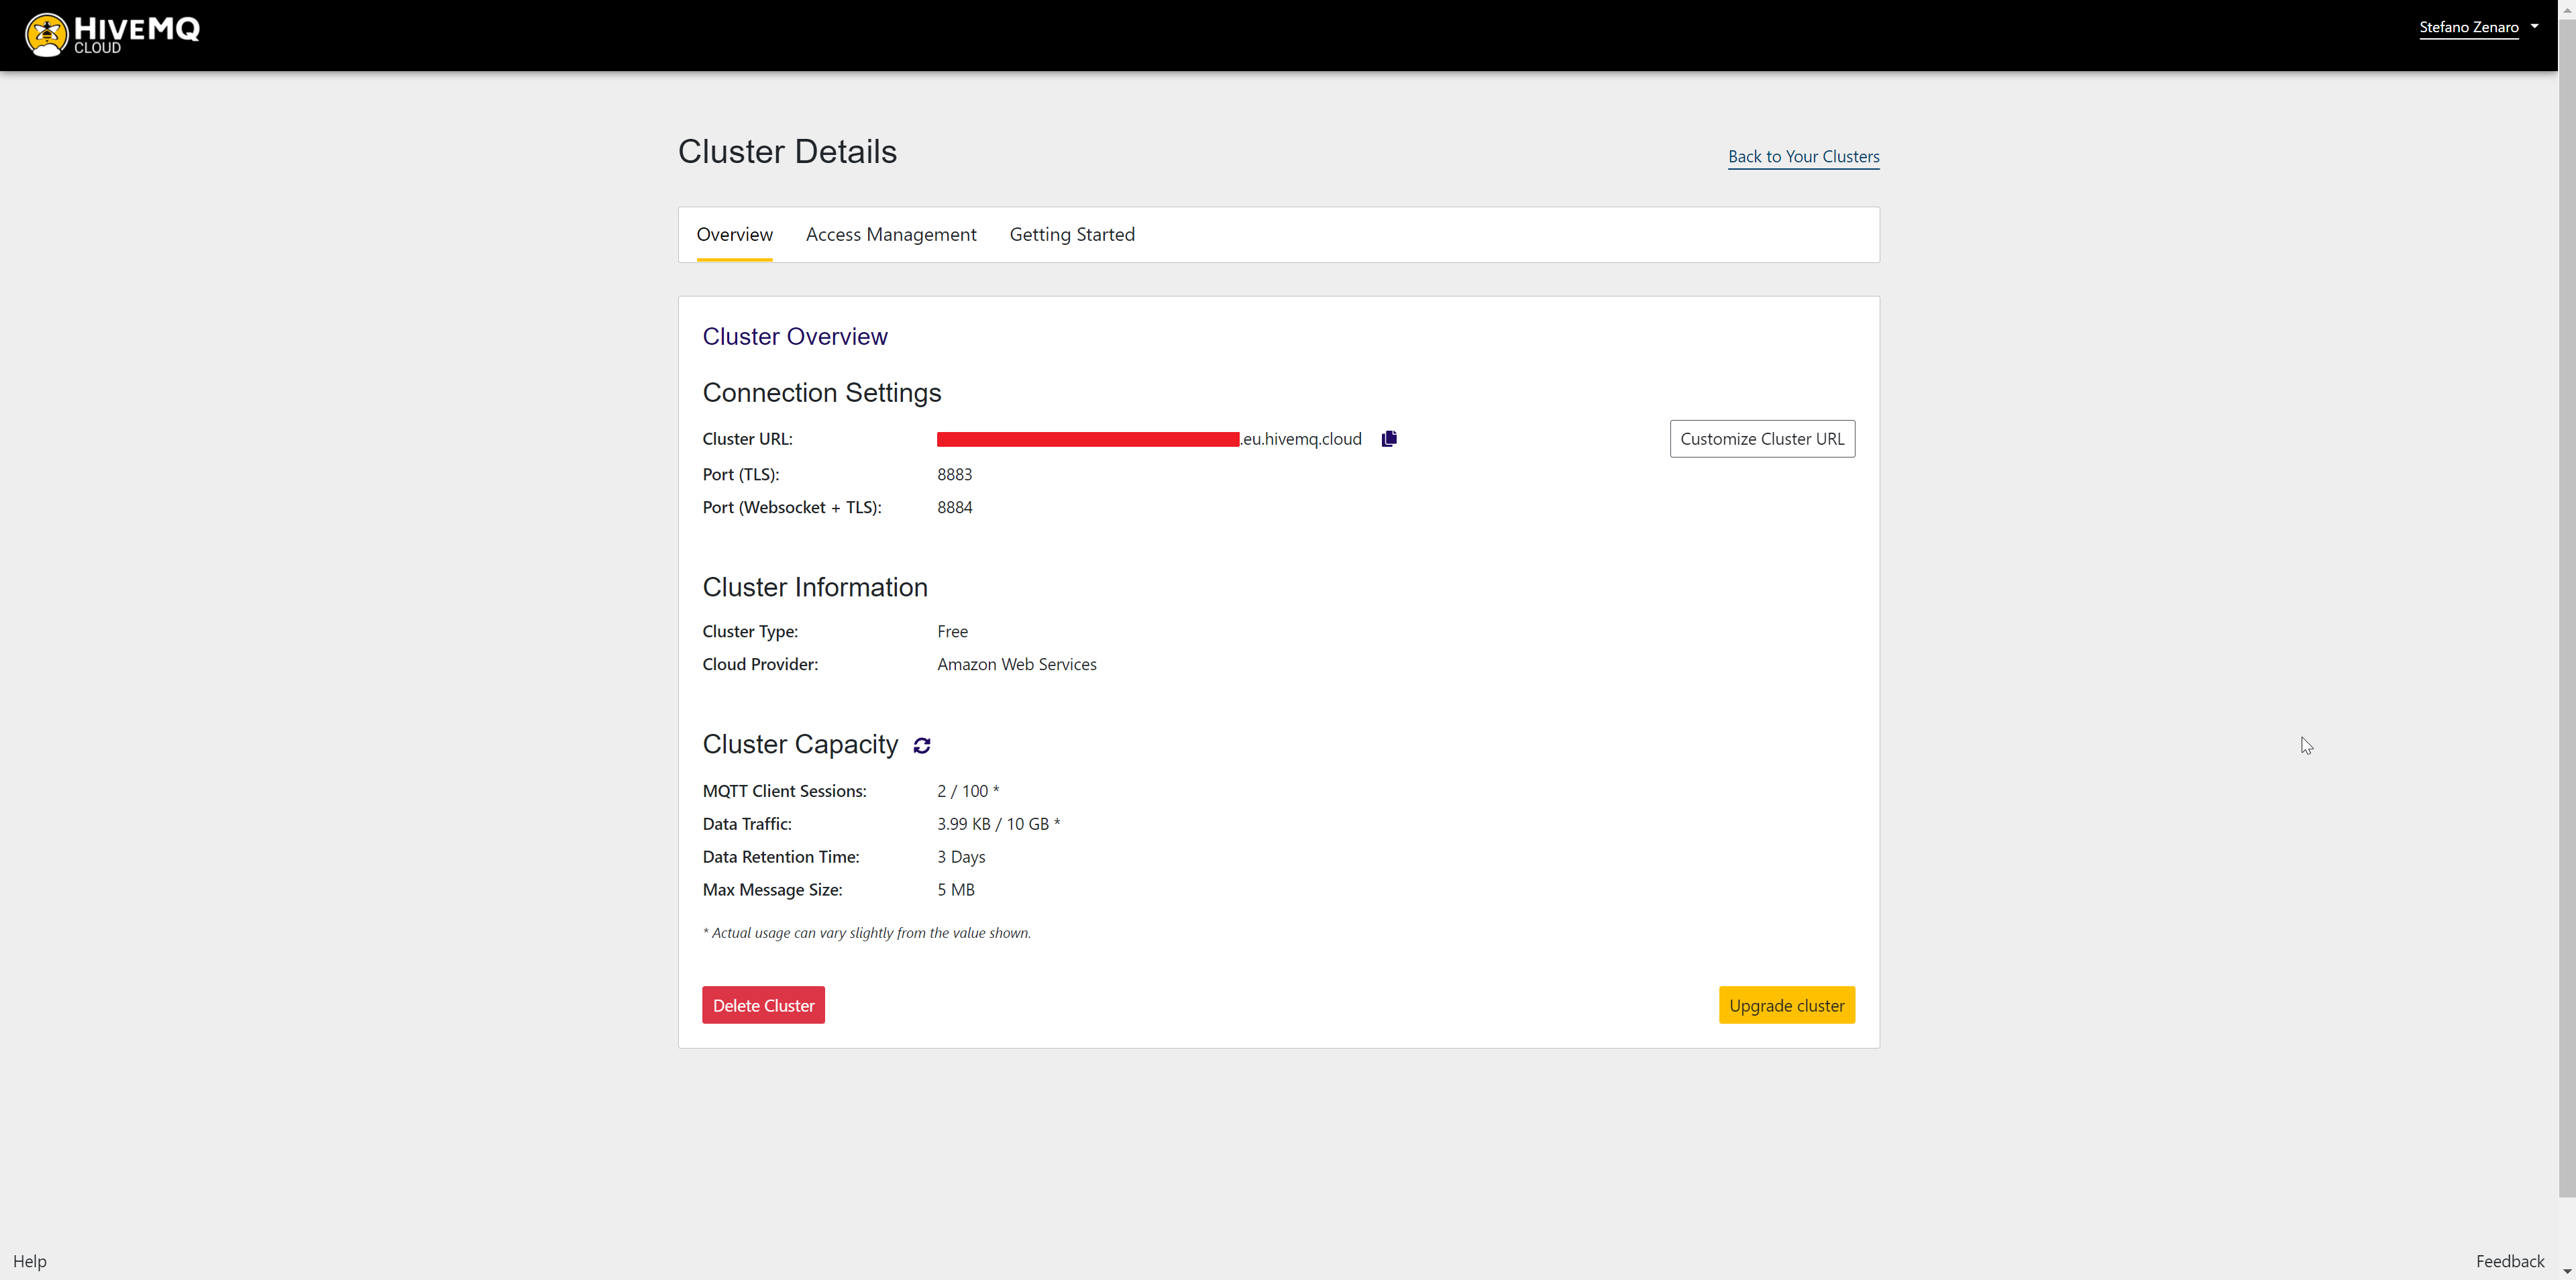
\includegraphics[width=\textwidth,height=\textheight,keepaspectratio]{assets/hivemq_clusterdetails}

Spostandosi nella tab "Access Management" e' possibile creare e vedere account utilizzati dai dispositivi per connettersi al Broker MQTT:

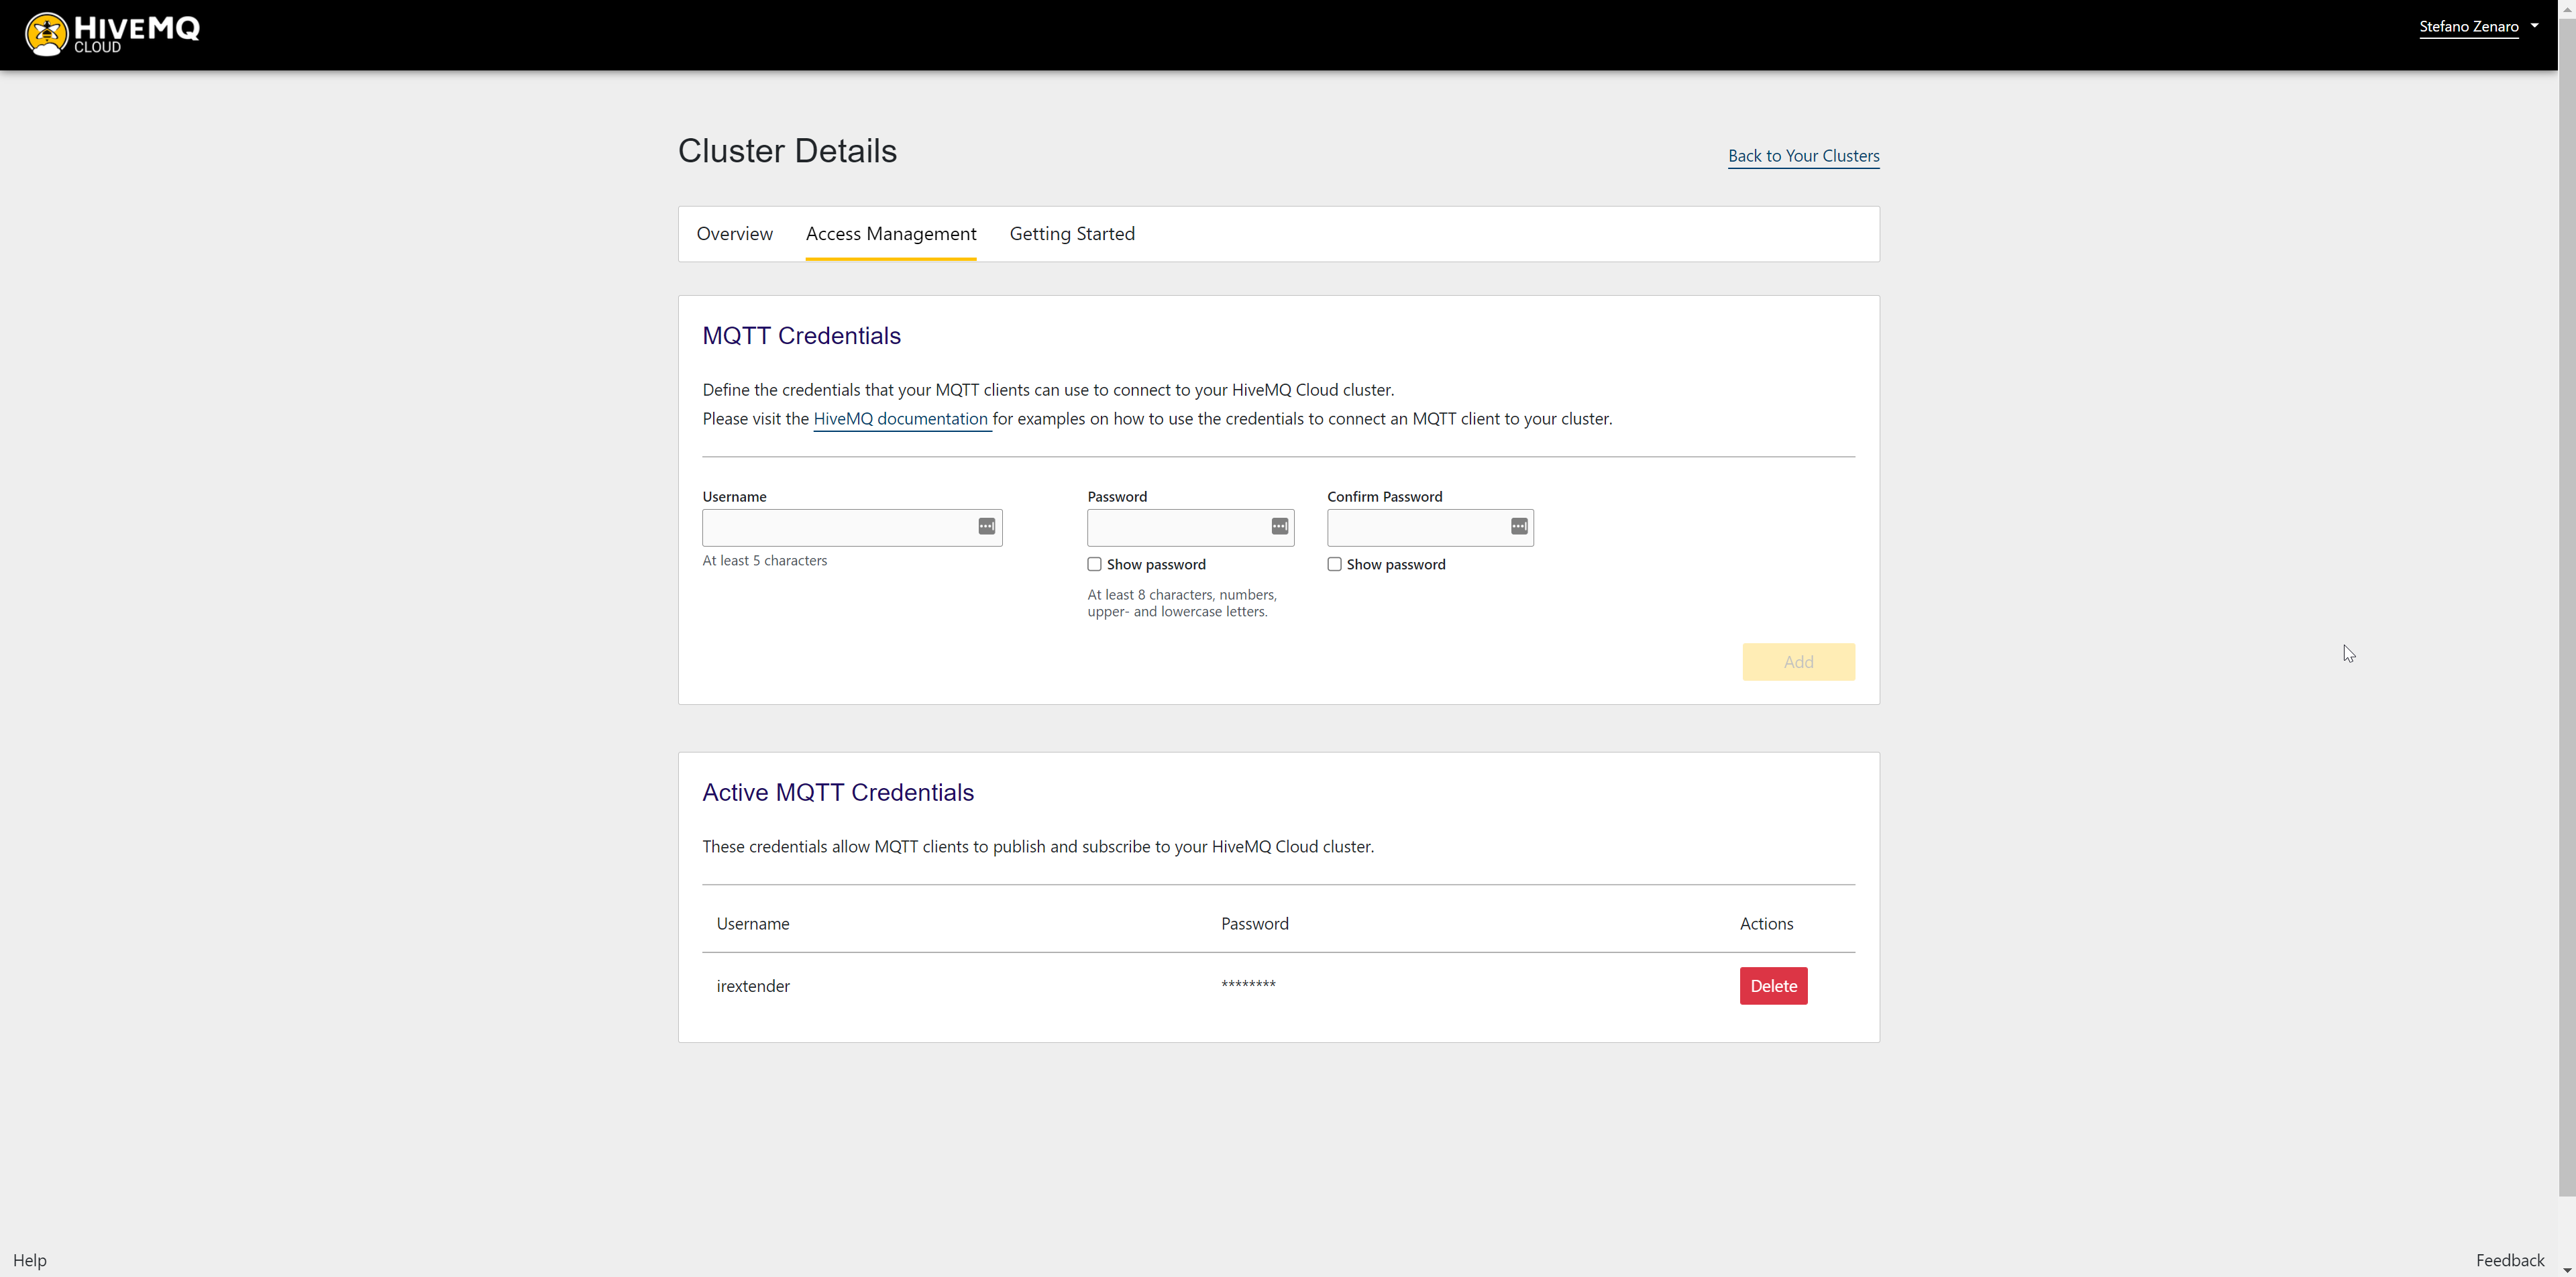
\includegraphics[width=\textwidth,height=\textheight,keepaspectratio]{assets/hivemq_access_management}

\end{document}
